\documentclass{beamer}
\usepackage{amsmath,amssymb,latexsym,array,fancyheadings,mathdots}
\usepackage{algorithm,algorithmic}
\usepackage{hyperref}
\usepackage{color}
\usepackage{tabularx}
\usepackage[all]{xy}
\usepackage{qtree}
\usepackage{gitinfo2}

%% RCS
%\usepackage{rcs}

%% Colors
\definecolor{darkgreen}{rgb}{0,.4,0}
\definecolor{darkred}{rgb}{.5,0,0}
\definecolor{darkmagenta}{rgb}{.5,0,.5}
\definecolor{orange}{rgb}{1,.5,0}
\definecolor{lightblue}{rgb}{0.122,0.016,0.855}
\definecolor{darkocre}{rgb}{0.471,0.298,0.008}

\usetheme{default}

%% New Theorems
\newtheorem{thm}{Theorem}
\newtheorem{exm}[thm]{Example}
\newtheorem{cor}[thm]{Corollary}
\newtheorem{propo}[thm]{Proposition}
\newtheorem{lem}[thm]{Lemma}
\newtheorem{clm}[thm]{Claim}
\newtheorem{exr}[thm]{Exercise}
\newtheorem{dfn}[thm]{Definition}

%% New commands
\newcommand{\classfont}{\mathsf}
\newcommand{\ATM}{\classfont{A}_{\mathrm{TM}}}
\newcommand{\MTF}{\mathrm{MTF}}
\newcommand{\OPT}{\mathrm{OPT}}
\newcommand{\ALG}{\mathrm{ALG}}
\newcommand{\ALGNAIVE}{\mathrm{ALG}_{\text{na{\"\i}ve}}}
\newcommand{\LRU}{\mathrm{LRU}}
\newcommand{\FIFO}{\mathrm{FIFO}}
\newcommand{\FWF}{\mathrm{FWF}}
\newcommand{\LFD}{\mathrm{LFD}}
\newcommand{\true}{\mathsf{T}}
\newcommand{\false}{\mathsf{F}}
\newcommand{\also}{\wedge}
\newcommand{\lra}{\leftrightarrow}
\newcommand{\tc}{\textcolor}
\newcommand{\df}[1]{\textcolor{red}{\em #1}}
\newcommand{\highlight}[1]{\textcolor{orange}{\em #1}}
\newcommand{\hl}[1]{\textcolor{blue}{\em #1}}
\newcommand{\amp}{\texttt{\&}}
\newcommand{\hsh}{\texttt{\#}}
\newcommand{\ra}{\rightarrow}
\newcommand{\longra}{\longrightarrow}
\newcommand{\Ra}{\Rightarrow}
\newcommand{\rab}{{\rightarrow_\beta}}
\newcommand{\srab}{{\rightarrow^*_\beta}}
\newcommand{\aeq}{{=_\alpha}}
\newcommand{\order}{\mathrm{order}}
\newcommand{\rem}{\mathrm{rem}}
\newcommand{\IP}{\mathbf{IP}}
\newcommand{\PSPACE}{\mathbf{PSPACE}}
\newcommand{\thevalue}{\text{value}}
\newcommand{\pol}[1]{\mathbf{#1}}
\newcommand{\enc}{\text{Enc}}
\newcommand{\xor}{\oplus}
\newcommand{\zo}{\{0,1\}}
\newcommand{\SOPT}{S_{\mathrm{opt}}}
\newcommand{\la}{\leftarrow}
\newcommand{\myurl}[1]{\textcolor{darkgreen}{\url{#1}}}
\newcommand{\myhref}[2]{\textcolor{darkgreen}{\href{#1}{#2}}}
\newcommand{\qaccept}{q_{\mathrm{accept}}}
\newcommand{\qreject}{q_{\mathrm{reject}}}
\newcommand{\opt}{\text{\sc Opt}}
\newcommand{\tr}{\mathrm{tr}}
\newcommand{\csanky}{p^{\textsc{csanky}}}
\newcommand{\berk}{p^{\textsc{berk}}}

%% Algorithms package customization
\renewcommand{\algorithmicrequire}{\textbf{Pre-condition:}} 
\renewcommand{\algorithmicensure}{\textbf{Post-condition:}} 
\algsetup{indent=3em}

\input{prooftree}

%% including/excluding pauses
\newcommand{\ifpause}{\iftrue} % for including pauses
%\newcommand{\ifpause}{\iffalse} % for excluding pauses

%% 2nd or 3rd edition
\newif\ifthird
\thirdtrue
%\thirdfalse

%disables usefoottemplate
\setbeamertemplate{navigation symbols}{}
%\setbeamertemplate{footline}% 
%{\strut\quad\tiny 
%\begin{minipage}{3cm}
%Cryptography - Michael Soltys
%\today\ {\tt v\RCSRevision}
%\end{minipage}\hfill
%\insertsection\
%- \insertframenumber/\inserttotalframenumber\quad\strut}

\newcommand{\mytitle}{Computational Foundations \\ Section 9.3}
\newcommand{\mychpnr}{9}
%% Title page contents
\title{Intro to Analysis of Algorithms \\ \mytitle \\  Chapter \mychpnr}
\author{Michael Soltys}
\date{\textcolor{darkgreen}{\tiny\tt 
[ {\bf Git} Date:\gitAuthorDate\ 
Hash:\gitAbbrevHash\ 
Ed:\ifthird
3rd
\else
2nd
\fi]}}
\institute{CSU Channel Islands}

\setbeamertemplate{footline}{
  \colorbox{white}{\color{black}\tt
     \begin{tabularx}{0.97\textwidth}{XXX}
          IAA Chp \mychpnr\ - Michael Soltys \copyright & 
          \hfill\today\ (\gitAbbrevHash; \ifthird ed3\else ed2\fi)
					\hfill\phantom{.} & 
          \hfill\insertsection\ - \insertframenumber/\inserttotalframenumber \\
      \end{tabularx}}}

\begin{document}

\mode<presentation>
{
}

\parskip 8pt

\section{Introduction}

\begin{frame}
\titlepage
\end{frame}


\begin{frame}
\begin{center}
\addtocounter{part}{1}
{\bf Section 9.3: \\ Regular languages}
\end{center}
\end{frame}

\begin{frame}
\df{Deterministic Finite Automaton (DFA)}  

$A=(Q,\Sigma,\delta,q_0,F)$

\begin{itemize}
\item  Finite set of states $Q$
\item  Finite set of input symbols $\Sigma$
\item  Transition fn $\delta:Q\times\Sigma\longrightarrow Q$;
given $q\in Q,a\in\Sigma$, $\delta(q,a)=p\in Q$ 
\item  Start state $q_0$
\item  A set of final (accepting) states.
\end{itemize}

To see whether $A$ accepts a string
$w$, we ``run'' $A$ on $w=a_1a_2\ldots a_n$ as follows:

$\delta(q_0,a_1)=q_1$, $\delta(q_1,a_2)=q_2$, until
$\delta(q_{n-1},a_n)=q_n$.  

Accept iff $q_n\in F$.
\end{frame}

\begin{frame}
\begin{minipage}{5cm}
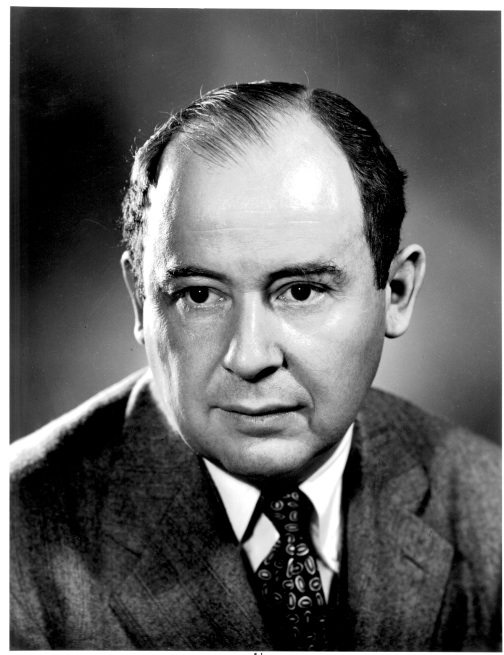
\includegraphics[width=4cm]{figures/JohnvonNeumann.jpg}
\end{minipage}
\begin{minipage}{5cm}
\myhref{http://en.wikipedia.org/wiki/John_von_Neumann}{John von Neumann} \\
\end{minipage}
\end{frame}

\begin{frame}
Consider $L=\{w|\text{ $w$ is of the form $x01y\in\Sigma^*$ }\}$ where
$\Sigma=\{0,1\}$.

We want to specify a DFA $A=(Q,\Sigma,\delta,q_0,F)$ that accepts all
and only the strings in $L$.

$\Sigma=\{0,1\}$, $Q=\{q_0,q_1,q_2\}$, and $F=\{q_1\}$.

\df{Transition diagram}
\begin{tabular}{l}
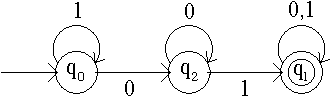
\includegraphics{figures/1.pdf}
\end{tabular}

\df{Transition table}
\begin{tabular}{c||c|c}
       & $0$   & $1$   \\\hline\hline
$q_0$  & $q_2$ & $q_0$ \\\hline
$q_1$  & $q_1$ & $q_1$ \\\hline
$q_2$  & $q_2$ & $q_1$
\end{tabular}
\end{frame}

\begin{frame}
\df{Extended Transition Function (ETF)}  given $\delta$, its ETF is
$\hat\delta$ defined inductively:

Basis Case: $\hat\delta(q,\varepsilon)=q$

Induction Step: if $w=xa$, $w,x\in\Sigma^*$ and $a\in\Sigma$, then
$$
\hat\delta(q,w)=\hat\delta(q,xa)=\delta(\hat\delta(q,x),a)
$$ 
Thus: $\hat\delta:Q\times\Sigma^*\longrightarrow Q$.

$w\in L(A) \iff \hat\delta(q_0,w)\in F$

Here $L(A)$ is the set of all those strings (and only those) which are
accepted by $A$.
\end{frame}

\begin{frame}
\df{Language of a DFA:} $L(A)=\{w|\hat\delta(q_0,w)\in F\}$

Note that
\begin{itemize}
\item $A$ is a {\em syntactic} object
\item while $L(A)$ is a {\em semantic} object
\end{itemize}
Thus $L$ is a function that assigns a {\em meaning} or {\em
interpretation} to a syntactic object.

\df{Regular Languages:} $L$ is {\em regular} iff there exists a DFA
$A$ such that $L=L(A)$.
\end{frame}

\begin{frame}
\df{Nondeterministic Finite Automata (NFA)}

The transition function $\delta$ becomes a transition relation,
i.e., $\delta\subseteq Q\times\Sigma\times Q$, i.e., on the
same pair $(q,a)$ there may be more than one possible new state (or
none).

Equivalently, we can look at $\delta$ as
$\delta:Q\times\Sigma\longrightarrow\mathcal{P}(Q)$, where
$\mathcal{P}(Q)$ is the power set of $Q$.

$L_n=\{w|\text{ $n$-th symbol from the end is 1 }\}$ \\
What is an NFA for $L_n$
\begin{center}
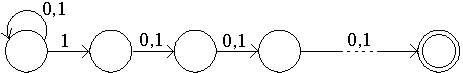
\includegraphics[width=7cm]{figures/2.pdf}
\end{center}
At least how many states does any DFA recognizing $L_n$ require?
\end{frame}

\begin{frame}
NFA with $\varepsilon$ transitions: $\varepsilon$-NFA:
$\delta:Q\times(\Sigma\cup\{\varepsilon\})\longrightarrow\mathcal{P}(Q)$

\begin{center}
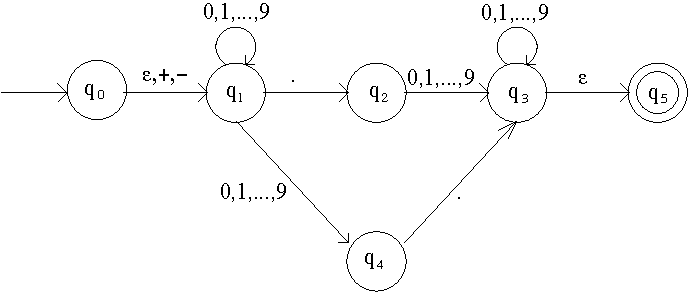
\includegraphics[width=8cm]{figures/3.pdf}
\end{center}
\end{frame}

\begin{frame}
To define $\hat\delta$ for $\varepsilon$-NFAs we need the concept of
$\varepsilon$-closure.

Given $q$, $\varepsilon$-close$(q)$ is the set of all states $p$ which
are reachable from $q$ by following arrows labeled by $\varepsilon$.

Formally, $q\in\varepsilon\text{-close}(q)$, and if
$p\in\varepsilon\text{-close}(q)$, and
$p\stackrel{\varepsilon}{\longrightarrow}r$, then
$r\in\varepsilon\text{-close}(q)$.

$\hat\delta(q,\varepsilon)=\varepsilon\text{-close}(q)$

Suppose $w=xa$, $\hat\delta(q,x)=\{p_1,p_2,\ldots,p_n\}$, \\
and $\cup_{i=1}^n\delta(p_i,a)=\{r_1,r_2,\ldots,r_m\}$, \\
then
$$
\hat\delta(q,w)=\cup_{i=1}^m\varepsilon\text{-close}(r_i)
$$
\end{frame}

\begin{frame}

{\bf Theorem:}  DFAs and $\varepsilon$-NFAs are equivalent.

{\bf Proof:}  Slightly modified subset construction.

$q^D_0=\varepsilon\text{-close}(\{q^N_0\})$

$\delta_D(R,a)=\cup_{r\in R}\varepsilon\text{-close}(\delta_N(r,a))$

Given a set of states $S$, its $\varepsilon$-closure is the union of
the $\varepsilon$-closures of its members.  

The states of $D$ are those subsets $S\subseteq Q_N$ which are equal
to their $\varepsilon$-closures. 

{\bf Corollary:}
A language is regular \\
$\iff$ it is recognized by some DFA \\
$\iff$ it is recognized by some NFA \\
$\iff$ it is recognized by some $\varepsilon$-NFA
\end{frame}

\begin{frame}

Union: $L\cup M=\{w|w\in L\text{ or }w\in M\}$ \\
Concatenation: $LM=\{xy|x\in L\text{ and }y\in M\}$ \\
Star (or closure): $L^*=\{w|w=x_1x_2\ldots x_n\text{ and }x_i\in L\}$

\df{Regular Expressions}

Basis Case: $a\in\Sigma,\varepsilon,\emptyset$

Induction Step: If $E,F$ are regular expressions, the so are
$E+F,EF,(E)^*,(E)$.

What are $L(a),L(\varepsilon),L(\emptyset),L(E+F),L(EF),L(E^*)$?

%Sipser 3.1.3(a)
Ex. Give a reg exp for the set of strings of 0s and 1s not
containing 101 as a substring:
$$
(\varepsilon+0)(1^*+00^*0)^*(\varepsilon+0)
$$
\end{frame}

\begin{frame}

{\bf Theorem:}  A language is regular iff it is given by some regular
expression.

{\bf Proof:}  reg exp $\Longrightarrow$ $\varepsilon$-NFA \&\
DFA $\Longrightarrow$ reg exp

$[\Longrightarrow]$

Use structural induction to convert $R$ to an $\varepsilon$-NFA with
3 properties:
\begin{enumerate}
\item  Exactly one accepting state
\item  No arrow into the initial state
\item  No arrow out of the accepting state
\end{enumerate}

Basis Case: $\varepsilon,\emptyset,a\in\Sigma$

\begin{center}
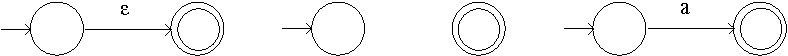
\includegraphics[width=10cm]{figures/4.pdf}
\end{center}
\end{frame}

\begin{frame}
Induction Step: $R+S,RS,R^*,(R)$

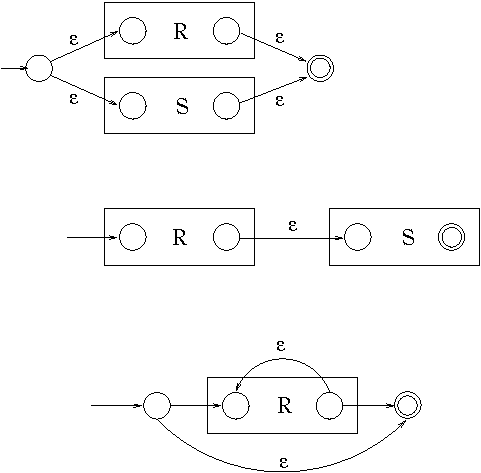
\includegraphics[height=6cm]{figures/5.pdf}
\end{frame}

\begin{frame}
$[\Longleftarrow]$ Convert DFA to reg exp.

{\bf Method 1}

Suppose $A$ has $n$ states.  $R^{(k)}_{ij}$ denotes the reg exp whose
language is the set of strings $w$ such that:
\begin{quote}
$w$ takes $A$ from state $i$ to state $j$ with all intermediate states
$\le k$
\end{quote}
What is $R$ such that $L(R)=L(A)$?

$R=R_{1j_1}^{(n)}+R_{1j_2}^{(n)}+\cdots+R_{1j_k}^{(n)}$
where $F=\{j_1,j_2,\ldots,j_k\}$

Build $R_{ij}^{(k)}$ by induction on $k$.

Basis Case: $k=0$, $R_{ij}^{(0)}=x+a_1+a_2+\cdots+a_k$ where
$i\stackrel{a_l}{\longrightarrow}j$ and $x=\emptyset$ if $i\neq j$ and
$x=\varepsilon$ if $i=j$
\end{frame}

\begin{frame}
Induction Step: $k>0$ 
$$
R_{ij}^{(k)}=\underbrace{R_{ij}^{(k-1)}}_{\text{path does not visit $k$}}
+\qquad
\underbrace{R_{ik}^{(k-1)}\left(R_{kk}^{(k-1)}\right)^*
R_{kj}^{(k-1)}}_{\text{visits $k$ at least once}}
$$

{\bf Method 2:}
DFA $\Longrightarrow$ G$\varepsilon$-NFA $\Longrightarrow$ Reg Exp

{\bf Generalized $\varepsilon$-NFA:} 
$$
\delta:(Q-\{q_{\text{accept}}\})\times
(Q-\{q_{\text{start}}\})\longrightarrow\mathcal{R}
$$
where the start and accept states are unique.  

$G$ accepts $w=w_1w_2\ldots w_n$, \underline{$w_i\in\Sigma^*$}, if
there exists a sequence of states
$$
q_0=q_{\text{start}},q_1,\ldots,q_n=q_{\text{accept}}
$$ 
such that for all $i$, $w_i\in L(R_i)$ where
$R_i=\delta(q_{i-1},q_i)$.
\end{frame}

\begin{frame}
When translating from DFA to G$\varepsilon$-NFA, if there is no arrow
$i\longrightarrow j$, we label it with $\emptyset$.  

For each $i$, we label the self-loop with $\varepsilon$.

Eliminate states from $G$ until left with just
$q_{\text{start}}\stackrel{R}{\longrightarrow}q_{\text{accept}}$:

\begin{center}
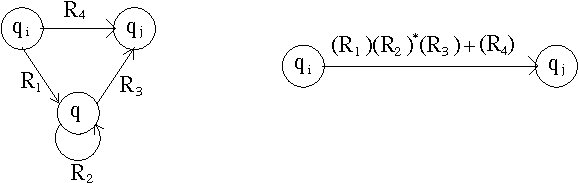
\includegraphics{figures/6.pdf}
\end{center}
\end{frame}

\begin{frame}

{\bf Algebraic Laws for Reg Exps}

$L+M=M+L$ (commutativity of $+$)\\
$(L+M)+N=L+(M+N)$ (associativity of $+$)\\
$(LM)N=L(MN)$ (associativity of concatenation) \\
$LM=ML$ ?

\bigskip

$\emptyset+L=L+\emptyset=L$ ($\emptyset$ identity for $+$) \\
$\varepsilon L=L\varepsilon=L$ ($\varepsilon$ identity for
concatenation) \\
$\emptyset L=L\emptyset =\emptyset$ ($\emptyset$ annihilator for
concatenation)

\bigskip

$L(M+N)=LM+LN$ (left-distributivity) \\
$(M+N)L=ML+NL$ (right-distributivity)
\end{frame}

\begin{frame}
$L+L=L$ (idempotent law for union) \\

\bigskip

Laws with closure:

$(L^*)^*=L^*$ \\
$\emptyset^*=\varepsilon$ \\
$\varepsilon^*=\varepsilon$ \\
$L^+=LL^*=L^*L$ \\
$L^*=L^++\varepsilon$

{\bf Test for Reg Exp Algebraic Law:}

To test whether $E=F$, where $E,F$ are reg exp with variables
($L,M,N,\ldots$), convert $E,F$ to concrete reg exp $C,D$ by
replacing variables by symbols.  If $L(C)=L(D)$, then $E=F$.

Ex. To show $(L+M)^*=(L^*M^*)^*$ replace $L,M$ by $a,b$, to obtain
$(a+b)^*=(a^*b^*)^*$.
\end{frame}

\section{Pumping Lemma}

\begin{frame}

{\bf Pumping Lemma:}  Let $L$ be a regular language.  Then there
exists a constant $n$ (depending on $L$) such that for all $w\in L$,
$|w|\geq n$, we can break $w$ into three parts $w=xyz$ such that:
\begin{enumerate}
\item  $y\neq\varepsilon$
\item  $|xy|\le n$
\item  For all $k\geq 0$, $xy^kz\in L$
\end{enumerate}

Proof:  Suppose $L$ is regular.  Then there exists a DFA $A$ such that
$L=L(A)$.  Let $n$ be the number of states of $A$.   Consider any
$w=a_1a_2\ldots a_m$, $m\geq n$:
$$
{}_{\displaystyle\stackrel{\uparrow}{p_0}}\overbrace{a_1
{}_{\displaystyle\stackrel{\uparrow}{p_1}}a_2
{}_{\displaystyle\stackrel{\uparrow}{p_2}}a_3
\ldots
a_i}^{x}
{}_{\displaystyle\stackrel{\uparrow}{p_i}}\overbrace{a_{i+1}
\ldots
a_j}^{y}
{}_{\displaystyle\stackrel{\uparrow}{p_j}}\overbrace{a_{j+1}
\ldots
a_m}^{z}{}_{\displaystyle\stackrel{\uparrow}{p_{m}}}
$$
\end{frame}

\begin{frame}
Ex. Show $L=\{0^n1^n|n\ge 0\}$ is {\em not} regular.

Suppose it is.  By PL $\exists p$.  Consider $s=0^p1^p=xyz$.  Since
$|xy|\le p$, $y\neq\varepsilon$, $y=0^j$, $j>0$.  And
$xy^2z=0^{p+j}1^p\in L$, which is a contradiction.

Ex. Show $L=\{1^p|\text{ $p$ is prime }\}$ is not regular.

Suppose it is.  By PL $\exists n$.  Consider some prime $p\geq n+2$. 

Let $1^p=xyz$, $|y|=m>0$.  So $|xz|=p-m$.

Consider $xy^{(p-m)}z$ which must be in $L$.  

But $|xy^{(p-m)}z|=|xz|+|y|(p-m)=(p-m)+m(p-m)=(p-m)(1+m)$

Now $1+m>1$ since $y\neq\varepsilon$, and $p-m>1$ since $p>n+2$ and
$m=|y|\le|xy|\le n$.  
So the length of $xy^{(p-m)}z$ is not prime, and
hence it cannot be in $L$ --- contradiction.
\end{frame}

\section{Myhill-Nerode Theorem}

\begin{frame}
$R$ is a \df{relation} on two sets $A,B$ if
$R\subseteq A\times B$.

e.g. $R=\{(m,n)|\text{ $m-n$ is even
}\}\subseteq\mathbb{Z}\times\mathbb{Z}$. \\
So $(3,5),(2,-4)\in R$, but $(-2,1)\notin R$.

$R$ is an \df{equivalence relation} if it is
\begin{enumerate}
\item  Reflexive: for all $a$, $(a,a)\in R$
\item  Symmetric: for all $a,b$, $(a,b)\in R\Rightarrow(b,a)\in R$
\item  Transitive: for all $a,b,c$, $(a,b)\in R$ and $(b,c)\in R$,
implies that $(a,c)\in R$.
\end{enumerate}
If $R$ is an equivalence relation, and $(a,b)\in R$, then we write
$a\equiv_R b$ or just $a\equiv b$.

Equivalence class: $[a]=\{x|x\equiv a\}$
\end{frame}

\begin{frame}

{\bf Theorem:}  For any equivalence relation:
\begin{enumerate}
\item  $a\in[a]$
\item  $a\equiv b\iff [a]=[b]$
\item  $a\not\equiv b$ then $[a]\cap[b]=\emptyset$
\item  any two equivalence classes are either equal or disjoint.
\end{enumerate}

{\bf Proof:}  3. prove the contra-positive: suppose
$[a]\cap[b]\neq\emptyset$, so there exists an $x\in[a]\cap[b]$.  

By definition, $x\equiv a$ and $x\equiv b$.  

By symmetry and transitivity, $a\equiv b$.
\end{frame}

\begin{frame}

$L\subseteq\Sigma^*$;
given $x,y\in\Sigma^*$ we say that they are \df{distinguishable} if
$\exists z\in\Sigma^*$ such that exactly one of $xz,yz$ is in $L$.

E.g., $L=\{w\in\{0,1\}^*|\text{ $w$ has an even number of 1s }\}$, and
$x=00,y=10$.  Then $x,y$ are distinguishable because letting $z=1$,
$xz=001\not\in L$ but $yz=101\in L$.

Given $L$, let $\equiv_L$ be the relation: $x\equiv_Ly$ iff $x,y$ are
{\em not} distinguishable.  Then $\equiv_L$ is an equivalence
relation.

{\bf Myhill-Nerode Theorem:}  $L$ is regular $\iff$ $\equiv_L$ has
{\em finitely many} equivalence classes.

Moreover, the number of states in the smallest
DFA recognizing $L$ is equal to the number of
equivalence classes of $\equiv_L$.
\end{frame}

\begin{frame}

{\bf Closure Properties of Regular Languages}

{\bf Union:} If $L,M$ are regular, so is $L\cup M$.

Proof: $L=L(R)$ and $M=L(S)$, so $L\cup M=L(R+S)$.

{\bf Complementation:} If $L$ is regular, so is $L^c=\Sigma^*-L$.

Proof: $L=L(A)$, so $L^c=L(A')$, where $A'$ is the DFA obtained from
$A$ as follows: $F_{A'}=Q-F_A$.

{\bf Intersection:} If $L,M$ are regular, so is $L\cap M$.

Proof: $L\cap M=\overline{\overline{L}\cup\overline{M}}$. 

{\bf Reversal:} If $L$ is regular, so is $L^R=\{w^R|w\in L\}$,
where $(w_1w_2\ldots w_n)^R=w_nw_{n-1}\ldots w_1$.

Proof:  Given a reg exp $E$, define $E^R$ by structural induction.
The only trick is that $(E_1E_2)^R=E_2^RE_1^R$.
\end{frame}

\begin{frame}

{\bf Homomorphism:} $h:\Sigma^*\longrightarrow\Sigma^*$, where
$h(w)=h(w_1w_2\ldots w_n)=h(w_1)h(w_2)\ldots h(w_n)$.

Ex. $h(0)=ab,h(1)=\varepsilon$, then $h(0011)=abab$.

$h(L)=\{h(w)|w\in L\}$

If $L$ is regular, then so is $h(L)$.

Proof:  Given a reg exp $E$, define $h(E)$.

{\bf Inverse Homomorphism:} $h^{-1}(L)=\{w|h(w)\in L\}$.

Proof:  Let $A$ be the DFA for $L$; construct a DFA for $h^{-1}(L)$ as
follows: $\delta(q,a)=\hat\delta_A(q,h(a))$.
\end{frame}

\begin{frame}

{\bf Complexity of converting among representations}

$\varepsilon$-NFA $\longrightarrow$ DFA is $O(n^32^n)$ \\
$O(n^3)$ for computing the $\varepsilon$ closures of all states --
Warshall's algorithm, and $2^n$ states

DFA $\longrightarrow$ NFA is $O(n)$ 

DFA $\longrightarrow$ Reg Exp  is $O(n^34^n)$ \\
There are $n^3$ expressions $R_{ij}^{(k)}$, and at each stage the size
quadruples (as we need four stage $(k-1)$ expressions to build one for
stage $k$)

Reg Exp $\longrightarrow$ $\varepsilon$-NFA is $O(n)$ \\
The trick here is to use an efficient parsing method for the reg exp;
$O(n)$ methods exist
\end{frame}

\begin{frame}

{\bf Decision Properties}

\begin{itemize}
\item  Is a language empty?

Automaton representation: Compute the set of reachable states from
$q_0$.  If at least one accepting state is reachable, then it is not
empty.

What about reg exp representation?

\item  Is a string in a language?

Translate any representation to a DFA, and run the string on the DFA.

\item  Are two languages actually the same language?

Equivalence and minimization of Automata.
\end{itemize}
\end{frame}

\begin{frame}

{\bf Equivalence and Minimization of Automata}

Take a DFA, and find an {\em equivalent} one with a {\em minimal}
number of states.

Two states are equivalent iff for all strings $w$,
\begin{quote}
$\hat\delta(p,w)$ is accepting $\iff$ $\hat\delta(q,w)$ is accepting
\end{quote}
If two states are not equivalent, they are {\em distinguishable}.

Find pairs of distinguishable states: Basis Case: if $p$ is accepting
and $q$ is not, then $\{p,q\}$ is a pair of distinguishable states.

Induction Step: if $r=\delta(p,a)$ and $s=\delta(q,a)$, where
$a\in\Sigma$ and $\{r,s\}$ are distinguishable, then $\{p,q\}$ are
distinguishable.
\end{frame}

\begin{frame}

{\bf Table Filling Algorithm}

A recursive algorithm for finding distinguishable pairs of states.

\begin{minipage}{5cm}
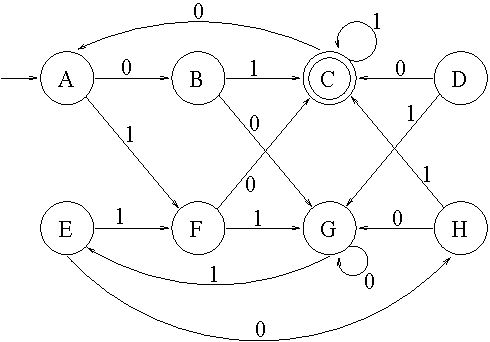
\includegraphics[width=5cm]{figures/7.pdf}
\end{minipage}
\begin{minipage}{5cm}
\begin{tabular}{|c|ccccccc}\hline
  & A & B & C & D & E & F & G \\\hline
B & x &   &   &   &   &   &   \\
C & x & x &   &   &   &   &   \\
D & x & x & x &   &   &   &   \\
E &   & x & x & x &   &   &   \\
F & x & x & x &   & x &   &   \\
G & x & x & x & x & x & x &   \\
H & x &   & x & x & x & x & x
\end{tabular}
\end{minipage}

Distinguishable states are marked by ``x''; the table is only filled
below the diagonal (above is symmetric).
\end{frame}

\begin{frame}

{\bf Theorem:} If two states are not distinguished by the algorithm, then
the two states are equivalent.

{\bf Proof:} Use the Least Number Principle (LPN): any set of natural
numbers has a least element.

Let $\{p,q\}$ be a distinguishable pair, for which the algorithm left
the corresponding square empty, and furthermore, of all such ``bad''
pairs $\{p,q\}$ has a shortest distinguishing string $w$.

Let $w=a_1a_2\ldots a_n$,
$\hat\delta(p,w)$ is accepting \&\ $\hat\delta(q,w)$ isn't.

$w\neq\varepsilon$, as then $p,q$ would be found out in the Basis Case
of the algorithm.

Let $r=\delta(p,a_1)$ and $s=\delta(q,a_1)$.  Then, $\{r,s\}$ are
distinguished by $w'=a_2a_3\ldots a_n$, and since $|w'|<|w|$, they
were found out by the algorithm.

But then $\{p,q\}$ would have been found in the next stage.
\end{frame}

\begin{frame}

{\bf Equivalence of DFAs}

Suppose $D_1,D_2$ are two DFAs.  To see if they are equivalent, i.e.,
$L(D_1)=L(D_2)$, run the table-filling algorithm on their ``union'',
and check if $q^{D_1}_0$ and $q^{D_2}_0$ are equivalent.

Complexity of the Table Filling Algorithm: there are
$n(n-1)/2$ pairs of states.  In one round we check all the pairs of
states to check if their successor pairs have been found
distinguishable; so a round takes $O(n^2)$ many steps.  If in a round
no ``x'' is added, the procedure ends, so there can be no more than
$O(n^2)$ rounds, so the total running time is $O(n^4)$.
\end{frame}

\begin{frame}

{\bf Minimization of DFAs}

Note that the equivalence of states is an equivalence relation.  We
can use this fact to minimize DFAs.

For a given DFA, we run the Table Filling Algorithm, to find all the
equivalent states, and hence all the equivalence classes.  We call
each equivalence class a {\em block}.

In our last example, the blocks would be:
$$
\{E,A\},\{H,B\},\{C\},\{F,D\},\{G\}
$$
The states within each block are equivalent, and the blocks are
disjoint.

We now build a minimal DFA with states given by the blocks as follows:
$\gamma(S,a)=T$, where $\delta(p,a)\in T$ for $p\in S$.
\end{frame}

\begin{frame}
We must show that $\gamma$ is well defined; suppose we choose a
different $q\in S$.  Is it still true that $\delta(q,a)\in T$?

Suppose not, i.e., $\delta(q,a)\in T'$, so $\delta(p,a)=t\in T$, and
$\delta(q,a)=t'\in T'$.  Since $T\neq T'$, $\{t,t'\}$ is a
distinguishable pair.  But then so is $\{p,q\}$, which contradicts
that they are both in $S$.

Theorem: We obtain a minimal DFA from the procedure.

Proof:  Consider a DFA $A$ on which we run the above procedure to
obtain $M$.  Suppose that there exists an $N$ such that
$L(N)=L(M)=L(A)$, and $N$ has fewer states than $M$.

Run the Table Filling Algorithm on $M,N$ together (renaming the
states, so they don't have states in common).  Since $L(M)=L(N)$ their
initial states are indistinguishable.  Thus, each state in $M$ is
indistinguishable from at least one state in $N$.  But then, two
states of $M$ are indistinguishable from the same state of $N\ldots$
\end{frame}

\end{document}
